%File: formatting-instruction.tex
\documentclass[letterpaper]{article}
\usepackage{aaai}
\usepackage{times}
\usepackage{helvet}
\usepackage{courier}
\usepackage{graphicx}
\usepackage{xcolor}
\usepackage{natbib}
\usepackage{lmodern}
\usepackage[T1]{fontenc}
\bibliographystyle{aaai}
% Sudo Code packages
\usepackage[ruled, linesnumbered]{algorithm2e}

\usepackage{amsfonts}

\graphicspath{./..}

\frenchspacing
\setlength{\pdfpagewidth}{8.5in}
\setlength{\pdfpageheight}{11in}
\pdfinfo{
/Title (Reinforcement Learning: Parking lot)
/Author (Robert Horton)}
\setcounter{secnumdepth}{0}  
 \begin{document}

% The file aaai.sty is the style file for AAAI Press 
% proceedings, working notes, and technical reports.
%
\title{Reinforcement Learning\\ Artificial Neural Network: Valet Parking Lot }
\author{Robert Horton\\
UCCS\\
1420 Austin Bluffs Pkwy,\\
Colorado Springs, Colorado 80918\\
}
\maketitle

% ----------------------------------------------- Abstract
\begin{abstract}
\begin{quote}
In society when considering segregation amongst different groups, there seems to be just as many physiological phenomenons observed during this process but as there are seemingly counter intuitive revelations between relationships between the members of these different groups. Through coded implementation and passed parameters, an instance of a randomly generated graph can be made with different levels of how \textit{mixed} the members in the group are when considering two types of members.  When considering spacial awarness we also evaluate different percentage of \textit{open space} available in the simulated environment.  Then simulations of Schelling Segregations were performed with certain levels of \textit{contentedness}.  With multiple simulations and varying parameter values, we analyse dynamic graph interactions amongst members in a whole.
\end{quote}
\end{abstract}

% ----------------------------------------------- Introduction
\section{Introduction}

When first implementing \textit{Schelling Integration} into a coded simulation there were not many constraints or requirements given for the assignment.  There was some information included inside the book for the class  (\cite{10.5555/1805895}). Python was the chosen language to code this project in.   After some research there were several different works that had already been done on the subject (\cite{AdilMoujahid}).  With out looking to much into the code done for these coded simulation, a general structure was built to generate different environments and runs simulations.  To make sure that the code could be followed along easily and verbosity of how the code executed were output to a .log file and many graphs and plots were generated.  To turn on this verbose setting and get the most information from running the simulations, when ever calling this method or any abstract methods that call this, turn the verbosity keyword argument to \texttt{True}.\\

\begin{center}
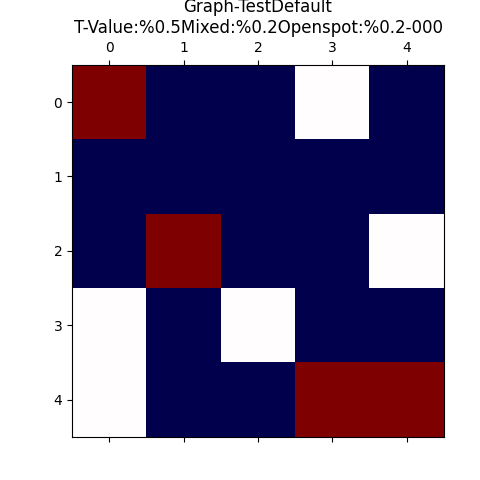
\includegraphics[scale=0.7]{./Images/TestExample_Figure_1.1}
Figure 1.1
\end{center}

% ----------------------------------------------- Implementation
\section{Implementation}  

To first implement the graph in which there would be different agents with spacial awareness, we used the NumPy library to generate two dimensional array's to represent the locations of each agents locations and their immediate neighbours.  Through this implementation we can evaluate different agents and keep track of where they are residing on the graphical grid.  On the graph there are two different types of agents, Red or Blue, with open spaces being the third option of what can occupy any of the array indexes at any point in time.  0 represents what are called open address or open spaces. The Red and Blue agents are also refereed to as Red or Blue residence being represented by the numerical value -1 and 1 respectively.  To generate these different graphs that would hold different values to essentially represent the 'Residence' of the 'City'.  There were a couple requirements in how generate the randomly placed residence and open spots.\\
To generate the City, there are two parameters that have to be chosen and set. The first one was the amount of open spot available in the City.  The second was how mixed the population should be in the city.  These two arguments can be used to generate a city which was done by first building a list that was populated with the different calculated numbers of each residence or open space to make up the entire city size.  The list was then shuffled and put into a NumPy array. Through a third key argument the simulation can be controlled to handle how each agent being evaluated reacts in its given environment.  The agent can be set to satisfied with its amount of same types direct Neighbors and choose to not move locations.  However, if the agent being evaluated does not have enough Neighbors of the same type, they will choice to move to a random address out of all the empty locations.  This was done through a simple method call that takes the index given for the residence under evaluation, and then index its direct neighbours.\\\\
Once the city has been generated and the contentedness levels for each residence are set, the simulation was left up to us to code in the way we thought best to evaluate the city for each iteration and its CTF value. The CTF was a metric discussed in class that was essentially the amount of cross type neighbours through the whole graph dived by the total number of total neighbours.  Therefore it is basically seeing how content the 'City' is with the current locations of where all the 'Residence' are located.  My first implementation was to choosing random locations and evaluate that way so I coded it to evaluate each residence one by one.  By the time I realized that the better to code this was to have contentedness level for each agent stored to either an object or dictionary it was to late.  So an implementation of evaluating each location in the graph in row major order.  After evaluating each index in the 'City' and possibly some of the same agents more than once, the CTF was calculated.  This implementation would move agents as evaluating so empty spots to move to could run out.  Evaluating each move seem to also maybe raise some concerns as sometimes it might get to the point where an agent has no where to move to, to make it content.  Although this would show convergence we have metrics to show this with a bit more tangibility.\\\\
Along with being able to control other key word arguments the user can choose the max number of iterations to perform on each simulation along with other attributes to keep track of graph logging and other verbose purposes. When evaluating direct neighbour and calling the method to check for neighbours we can count how many different type neighbours their are for that residence.  To make sure that direct neighbourhood spaces that are considered out of bounds we use a try block.  This way we can set the counter to not count the spaces that the residence cant move to.  The NumPy library was also used to randomly pick a empty location from a list of found locations that are holding 0.  By looking at the .logs files provided we can see that where ever an agent is discontent and by how much.  When turning the verbosity keyword argument to True, we can see all the information proved to show that this implementation works. To run multiple simulations and collect the average for each simulation run, the method \texttt{avd\_ctf} was created.  With this method, it runs 10 training sessions by default and returns the ending average for all the training sessions. There is a keyword available to control the number of runs test runs to training sessions to perform.\\\\
Through a passed list during initialization or by using one of the setter methods, we can select how often or at which points we would like to to capture and see points plotted for the simulation.  For the deliverable part 2 \& 3 a frequency global constant was given for the simulation to perform average runs with varying values.  The list of capture points also controls the resolution on the .gif generated by the simulations. 
 
% ----------------------- Execution 
\subsection{Execution}

During execution the segregation amongst the map seemed to stay pretty consistent in between training sessions of the same original generated city and often would converge to looking very similar in where the clusters of 'Red' and 'Blue' residence were first densely populated.  Once we started to change the values for different parameters such as \texttt{red\_blue\_split} and \texttt{pct\_empty} completely new random Cities were generated and populated. The shapes of the segregated Cities would lose their consistent shape in between varying values for this reasons.  This is not to say that it would or would not if we simply took out residence or change the colour amongst the residence but something that could be implemented further to keep the consistent shape of the randomized populated city would be interesting to further research.  When implementing i Wasn't sure which way would be best, whether to pick randomnly thorugh the city and evaluate residence ro to go through each one for each iteration.  So a keyword has been added to choose which method to execute during simulation.  This is done throuh the user input interface that ask the user whether to get one of the deliverable out puts or all of them.  This helped keep the program from crashing when asking it to develop only one deliverable.  The All option was added and for every 10 runs it seems to fail on the last deliverable.  Once a proper output has been chosen, the user input interface then ask ths user to choose which method of execution to run.   To run in iteration over each resident, choose 'Row' to choose at random choose "Random".  Row major seems to be the fastest and get higher results for CTF.

% ----------------------- Analyisis 
\subsection{Analyisis}

When performing training sessions with varying mixed population values It seemed like there didn't really seem to be much difference when keeping the rest of the values constant all though this could be different with other varying open percentage and open space values.  Signs of segregation would show them selves through various runs but still seem to have the same max CTF and rate of convergence with some slight differnces between training simulations.  When looking at the varying valued simulations it seemed to show that the CTF between runs would seem to drop as the mixed percetage got closed to 0.5 compared to the other values that seem to have a slightly higher CTF value.  Figure 1.2 and this suggests that the more offset a population is the higher the CTF value will be which makes sense.\\ 
\begin{center}
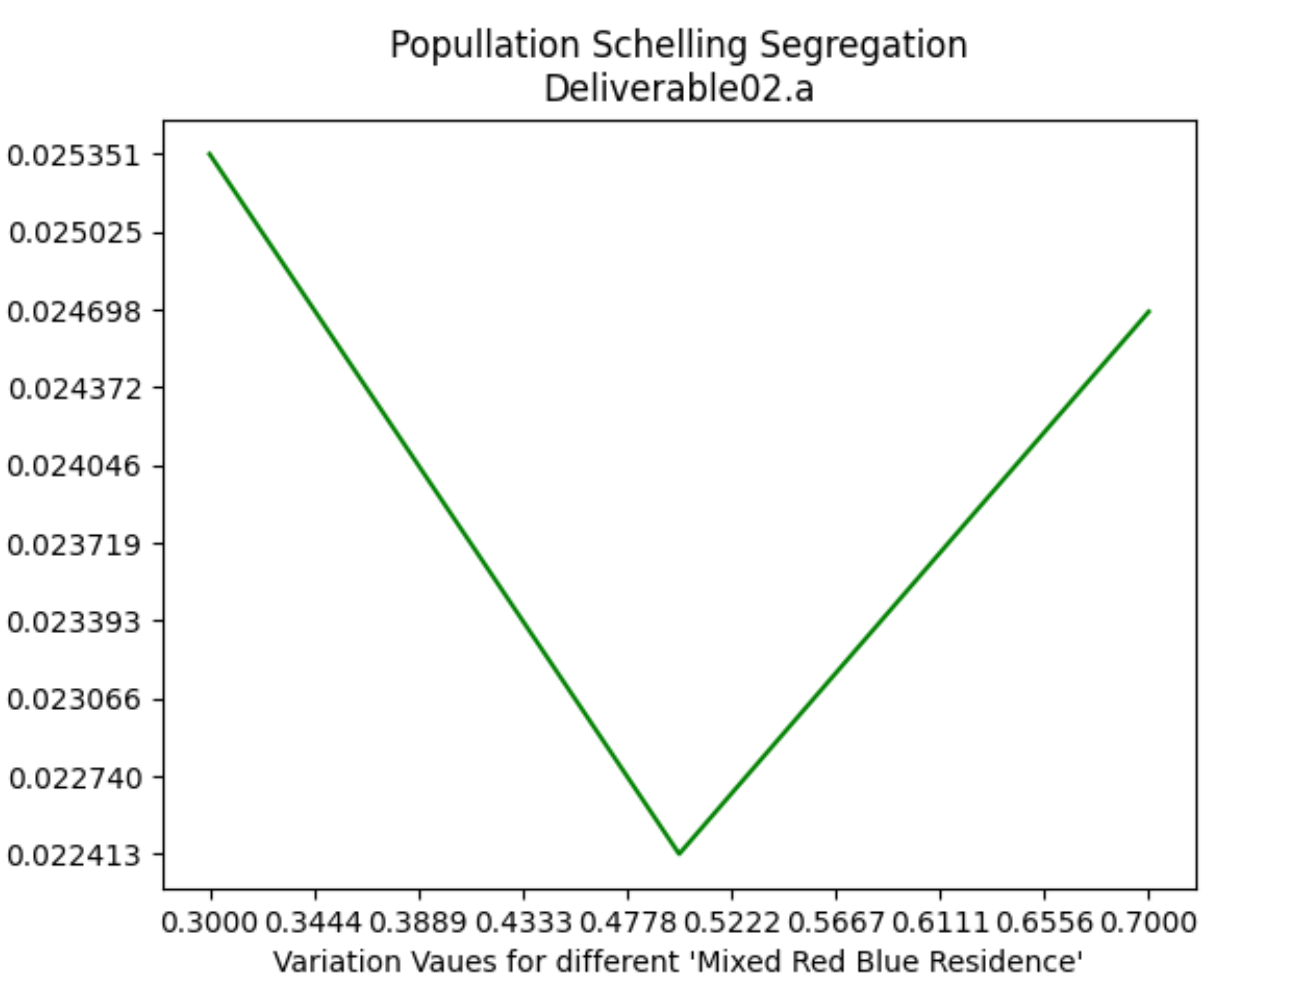
\includegraphics[scale=0.6]{./Images/DeliverableA_Figure1.2}
Figure 1.2
\end{center}
As for the training sessions for varying t-values we seem where the CTF  has a almost linear decline as the t-value gets higher.  Ultimately these values give us the lost CTF out of all the other combinations or varying values. This suggests that to achieve a high CTF, the t-values that are closer to higher are the best value to achieve higher CTF values and more segregation. \\
\begin{center}
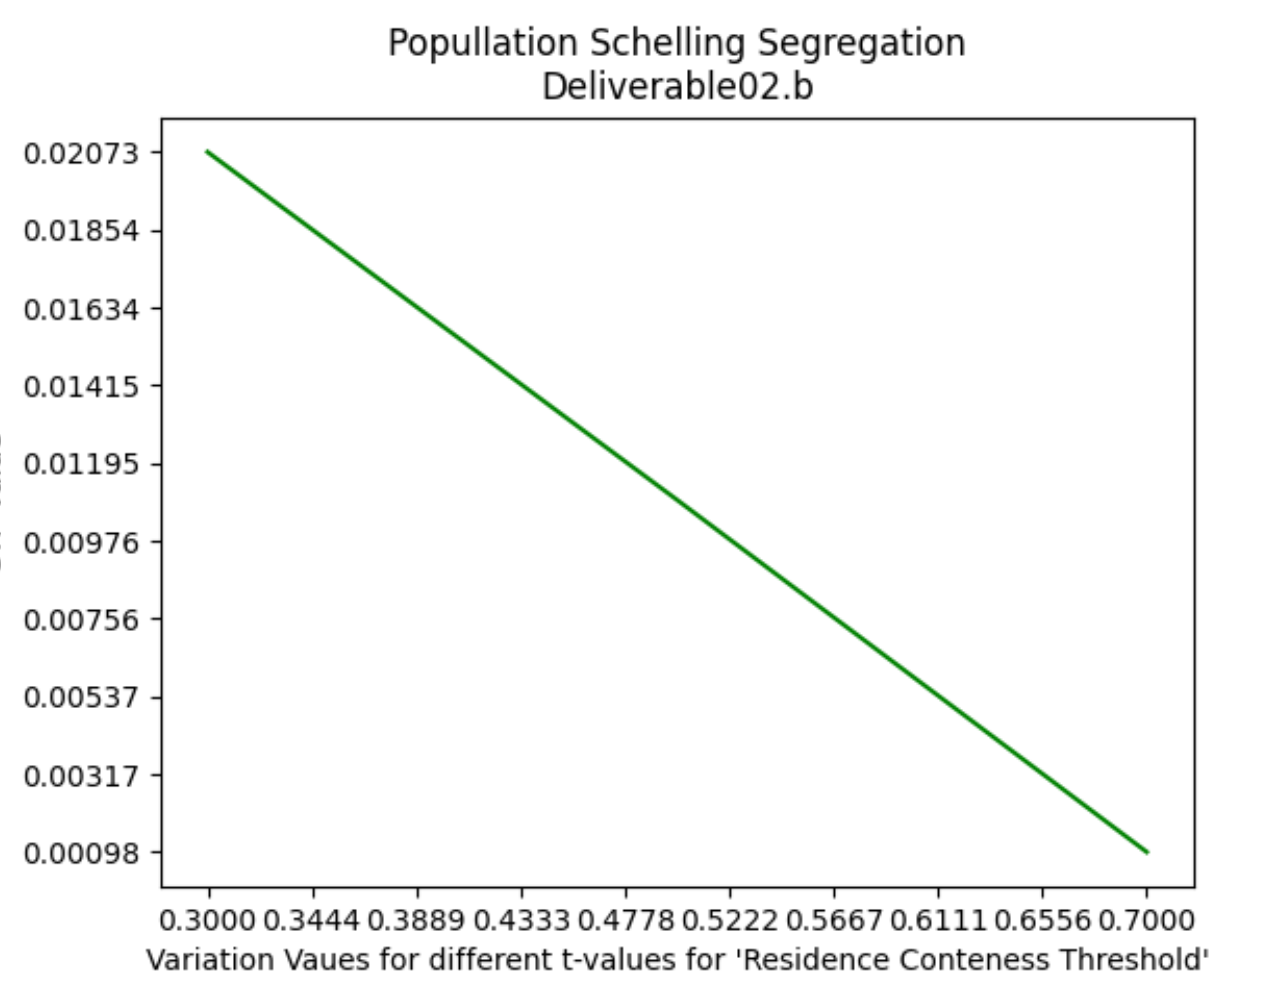
\includegraphics[scale=0.6]{./Images/Deliverableb_Figure1.3} 
Figure 1.3
\end{center}
When performing the different training sessions with varying open space percentage we would still see clusters start to form but when the open space got big enough for most neighbours to be content with their environment we start to see very little to no clusters.  Any clusters that do form do not seem to be very dense and will have lots of open hole in the collection of like type neighbours.  This probably also led to there being little to no spaces to move to and their fore were forced to either move randomly or stay were that are.  When looking at CTF values we see a spike when the percentage gets to 0.5 .  In Figure 1.4 we that the CTF values go down a little bit more when closer 0.7 then when using .02 percent open spots.  As for 0.5 we see it go to the highest CTF.  Ultimately less to half percentage ended in higher CTF values.  In the end their usually tended to be more open space often leading to very scattered less dense collection of like type neighbours. \\
\begin{center}
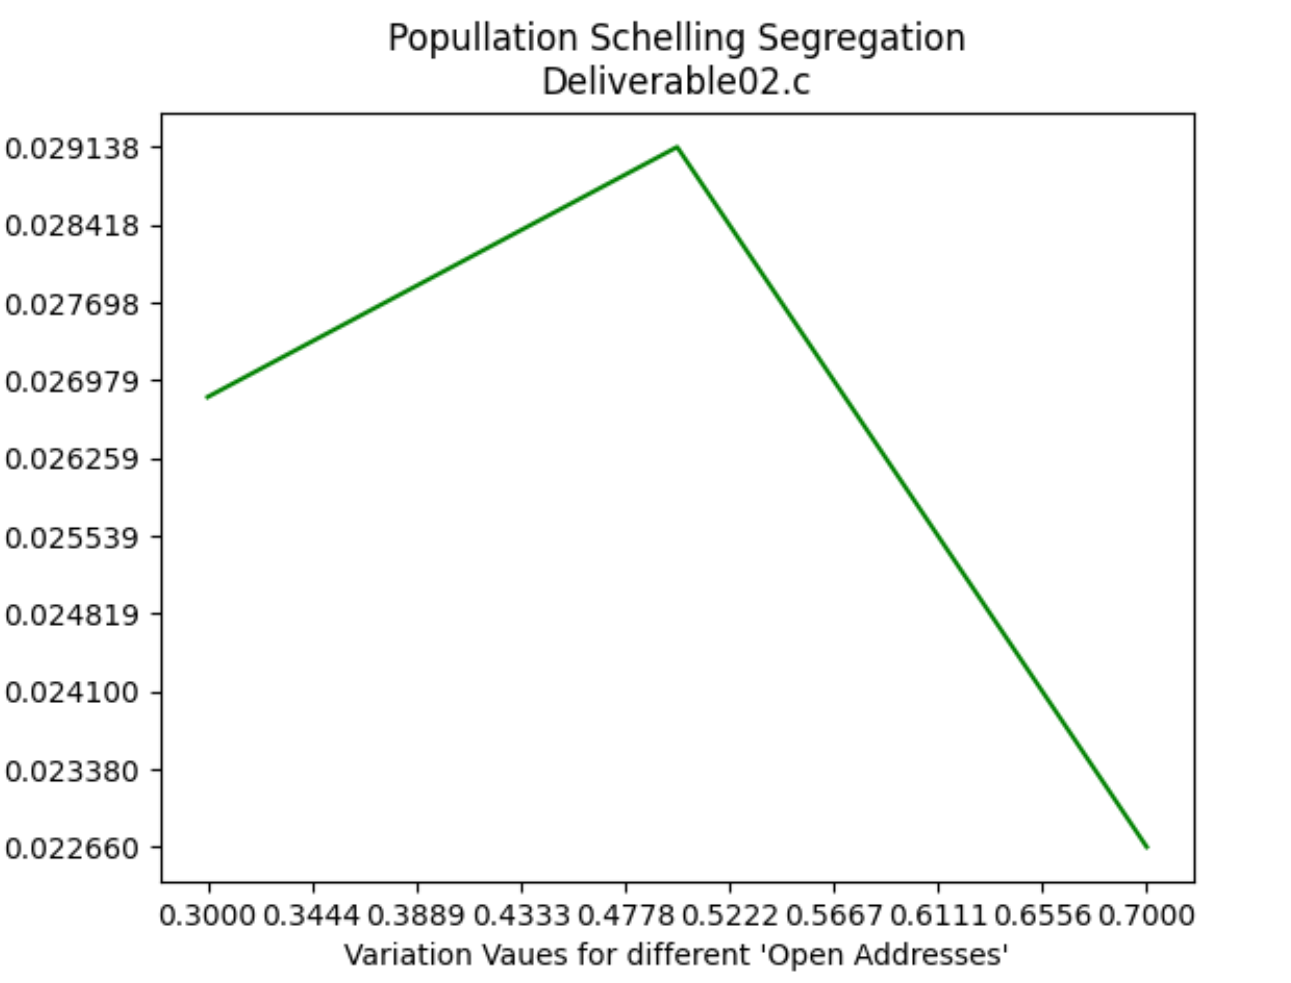
\includegraphics[scale=0.6]{./Images/DeliverableC_Figure1.4}
Figure 1.4
\end{center}

% ----------------------------------------------- Conclusion
\section{Conclusion}
In conclusion i learned alot about this subject and the interesting correlation it has with different values.  I learned alot about rendering gifs and using the NumPy library.  Ultimately I learned how to try to think about coding more efficient and after coding this up twice I still ran into or thought of different ways i could have implemented it better.  In the end the higher the t-value generally the loser the CTF.

% ----------------------------------------------- References 

\bibliography{ArticleTemplate}

\end{document}